\section{Интерферометр Майкельсона. Фурье-спектрометр. Применение интерферометров в научных исследованиях}

\subsection{Интерферометр Майкельсона}

Схема интерферометра представлена на рисунке. 

\begin{figure}[H]
	\centering
	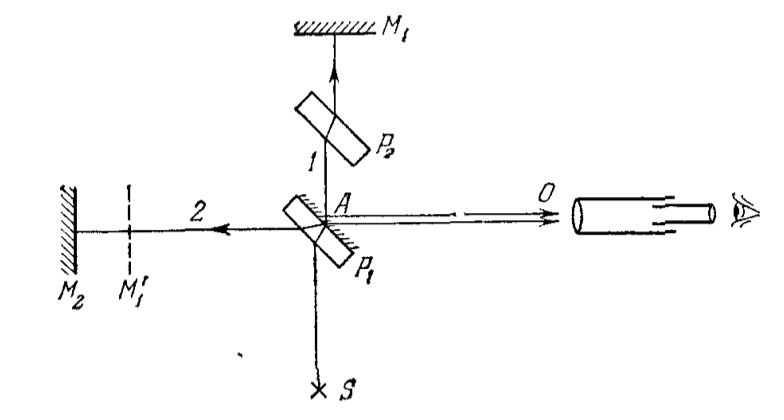
\includegraphics[width=\linewidth]{26_1}
	\caption{Интерферометр Майкельсона}
\end{figure}

Приведем краткое описание:

Свет от некоторого протяженного источника $S$ попадает на плоскопараллельную полупрозрачную пластинку $P_1$. Она разделает попавший на нее пучок на два, первый и второй соответственно. Первый пучок, после прохождения пластинки, отражается обратно \textbf{статичным} зеркалом $M_1$, после чего частично отражается от пластинки $P_1$ в указанном направлении. Второй же пучок, отразившись от границы пластинки $P_1$, направляется к зеркалу $M_2$, после чего проходит через пластинку $P_1$ и идет совместно с пучком 1. Отметим, что второй пучок проходит пластину $P_1$ трижды. Чтобы исключить получающуюся из-за этого разность фаз, на пути первого пучка ставят пластинку $P_2$, идентичную $P_1$.

Пусть $M_1'$ --- изображение зеркала $M_1$ в отражающей плоскости пластинки $P_1$. Тогда происходящая интерференция равносильна интерференции в воздушном слое между $M_1'$ и $M_2$. Разность хода между лучами составляет $\Delta = 2 d\cos \phi$, где $d$ --- толщина слоя, $\phi$ --- угол падения. Если слой плоскопараллелен, то мы получим интерференционные кольца с центром в точке схождения лучей, нормально отраженных от поверхностей $M_1'$ и $M_2$. Этому направлению соответствует максимальная разность хода $\Delta = 2 d$, значит максимальный порядок интерференции будет в центре. При увеличении $d$ полосы будут перемещаться от центра; при увеличении зазора на $d = \lambda/2$, произойдет смещение картины на одну полосу (т.е. на место светлой полосы снова придет светлая), т.к. $\Delta = \lambda$. Если же мы измени угол падения, то разность хода изменится на $\Delta = 2 d \sin\phi \Delta\phi$. Полосы получаются чем шире, чем меньше $d$, т.е. при $d = 0$ мы получим равномерное освещение.

Интерферометр использовался, например, при проведении  \href{https://elementy.ru/trefil/21167/Opyt_MaykelsonaMorli}{опыта Майкельсона -- Морли}, в ходе которого было установлено отсутствие движения Земли относительно эфира.

\subsection{Фурье-спектрометр}

Схема спектрометра представлена на рисунке. 

\begin{figure}[H]
	\centering
	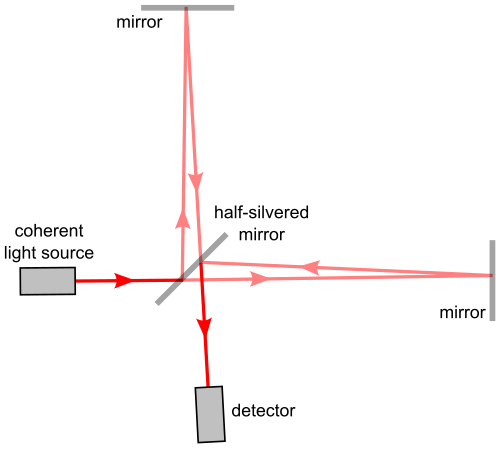
\includegraphics[width=\linewidth]{26_2}
	\caption{Фурье=спектрометр}
\end{figure}

Приведем краткое описание:

Основой спектрометра является интерферометр Майкельсона (только он тут почему-то без второй пластины, ха-ха). Предположим, что у нас есть некоторый когерентный источник излучения с длиной волны $\lambda$. Когда разность хода лучей в спектрометре оказывается равной $\lambda/2$, интенсивность регистрируемого света оказывается близкой к нулю. При перемещении правого зеркала интерферометра Майкельсона разность хода лучей изменяется, изменяется и интенсивность света, регистрируемая приёмником. Очевидно, что интенсивность света максимальная, когда разность хода лучей будет кратна длине волны $\lambda$.

При перемещении зеркала с постоянной скоростью на выходе приёмника будет наблюдаться электрический сигнал синусоидальной формы. Притом период синусоиды зависит от длины волны источника, а амплитуда от интенсивности источника.

Теперь представим, что на входе некогерентный источник. Каждая длина волны в спектре источника света будет давать свою синусоиду на выходе приёмника. Таким образом, на выходе приёмника мы получаем сложный сигнал. При выполнении над полученным сигналом обратного преобразования Фурье получаем спектр входного электрического сигнала, который также является спектром излучения источника (то есть интенсивность излучения источника на различных длинах волн).

За счет этого можно проводить спектральные анализы для выявления состава газов или жидкостей. Каждый газ или жидкость имеет свой спектр поглощения проходящего через него излучения. Таким образом спектр на входе интерферометра будет иметь «провалы» на определённых длинах волн. После обратного преобразования Фурье получаем спектр поглощения, по которому достаточно просто определить присутствующие в анализируемом воздухе газы и их концентрацию.

\subsection{Применение интерферометров в научных исследованиях}

Фактически, интерферометр позволяет с большой точностью измерять расстояния, поэтому его можно применять для создания деталей, изготовление которых требует высокой точности (сдвиг в интерференционной картине будет виден даже при небольшом отклонении).

Интерференционные методы позволяют с высокой точностью выявлять очень малые изменения показателя преломления среды, которые влияют на изменение оптической длины пути, а значит, влекут за собой изменение интерференционной картины.

Можно также измерять и углы.